\documentclass[compress,red]{beamer}
\usetheme{Warsaw}
\useoutertheme[subsection=false]{smoothbars}

\usepackage{helvet}
\usepackage{graphicx}
\usepackage{booktabs}
\usepackage{hyperref}
\usepackage{url}

\usepackage{remreset}% tiny package containing just the \@removefromreset command
\makeatletter
\@removefromreset{subsection}{section}
\makeatother
\setcounter{subsection}{1}

\title[Managing equipment at CERN]%
	{A strategy for managing diverse equipment\\
	in the CERN controls group}
\author[Javier Serrano, David Cobas et al.]{%
	Javier Serrano, Juan David Gonz\'alez Cobas}
\date{FOSDEM'2012}

\begin{document}

% ------------------------------------------------------
\begin{frame}
\titlepage
\end{frame}

% ------------------------------------------------------
\begin{frame}
\frametitle{Software for Diverse Equipment}

We got ourselves a rather diverse hardware ecosyst...
\pause eeehh, sorry, \pause zoo
\pause
\begin{block}{Different species of hardware animals...}
\begin{itemize}
\pause\item analog I/O (ADCs, DACs, waveform generators)
\pause\item digital I/O
\pause\item timing boards (FD, TDC)
\end{itemize}
\end{block}
\pause
\begin{block}{...of diverse breed}
\begin{itemize}
\pause\item legacy stuff
\pause\item FMC boards
\end{itemize}
\end{block}

\pause Some order has to be imposed in the zoo.
\end{frame}

% ------------------------------------------------------
\begin{frame}
\frametitle{Unifying Themes}
\begin{block}{Wishbone-based drivers}
\begin{itemize}
\item covering the FMC family of boards
\item designed around the internal Wishbone bus
\item depending on enumeration of device cores
\end{itemize}
\end{block}
\begin{block}{\texttt{zio}: The Ultimate I/O}
\begin{itemize}
\item Linux kernel framework for I/O devices
\item oriented to high bandwidth applications
\end{itemize}
\end{block}


\end{frame}

% ------------------------------------------------------
\begin{frame}{The FMC family of boards}
\begin{itemize}
\item carriers in PCIe and VME form factors
\item simple mezzanines with electronics for ADCs, DACs, DIO and endless
    other applications
\item circuitry in the mezzanine
\item FPGA application logic in the carrier
\item \emph{logic in the FPGA is organized as a set of IP cores
    interconnected through an internal \textcolor{red}{Wishbone}}
    bus
\end{itemize}
\end{frame}
% ------------------------------------------------------
\begin{frame}{A typical data acquisition application: carrier}
\begin{center}
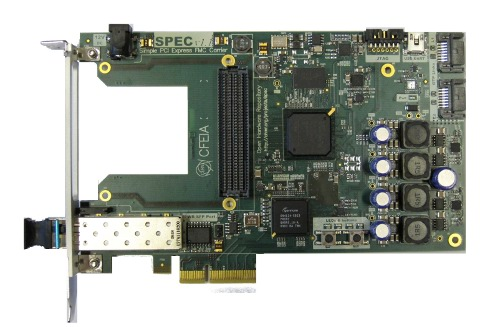
\includegraphics[height=0.6\textheight]{spec.pdf}
\end{center}
\centering
SPEC carrier board (\url{http://www.ohwr.org/projects/spec})
\end{frame}

% ------------------------------------------------------
\begin{frame}{A typical data acquisition application: mezzanine}
\begin{center}
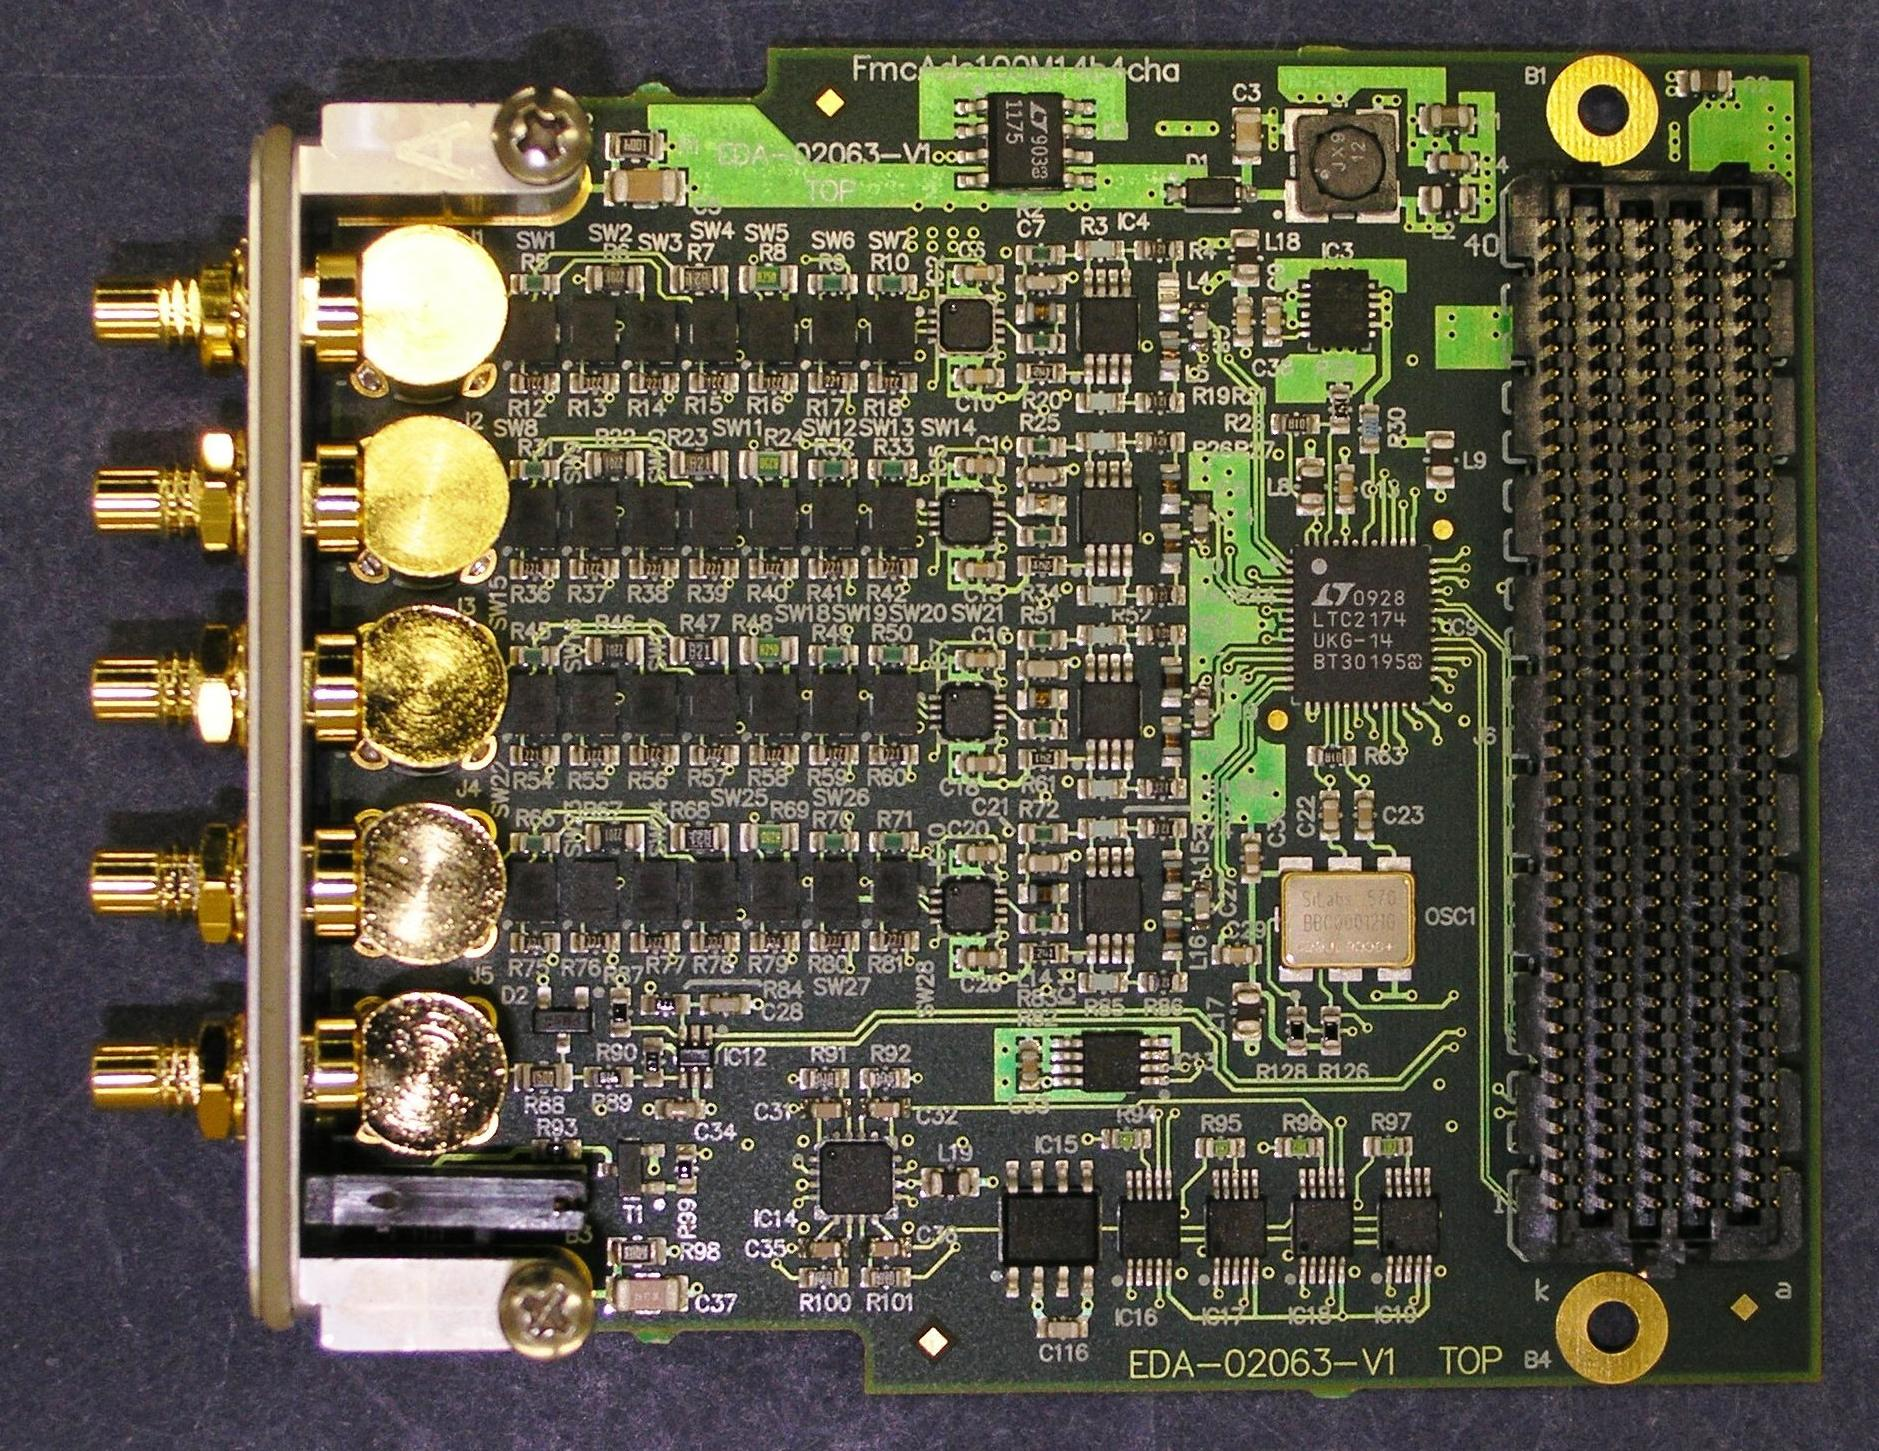
\includegraphics[rotate=180,height=0.7\textheight]{fmcadc.pdf}
\end{center}
\centering
FMA 100M4ch14b ADC
(\url{http://www.ohwr.org/projects/fmc-adc-100m14b4cha})
\end{frame}

% ------------------------------------------------------
\begin{frame}
\begin{figure}[t]
   \centering
   \includegraphics[width=80mm]{adcarch.pdf}
   \caption{Block diagram of the FMC slow ADC application.}
   \label{slow-adc}
\end{figure}
\end{frame}

% ------------------------------------------------------
\begin{frame}{Parts of the whole}
\begin{itemize}
\item Basic I${}^2$C interfacing to the mezzanine board.
\item Wishbone mastering.
\item DMA access to DDR3 memory in the carrier board.
\item Mezzanine-specific control logic (\emph{e.g.} ADC programming/setup).
\item Interrupt control.
\end{itemize}
\end{frame}

% ------------------------------------------------------
\begin{frame}{Drivers for the FMC family}
The main concepts for the design of these drivers are
\begin{itemize}
\pause
\item modular structure that reflects the core structure of the firmware
\pause
\item one-to-one mapping driver $\leftrightarrow$ core (usually)
\pause
\item ability to dynamically load bitstreams by application
\end{itemize}

\pause
On the whole, the driver for the carrier board acts as a basic firmware
loader and a bridge driver (with device enumeration
\emph{\`a la PCI)} between the host bus (PCIe, VME) and the FPGA
interconnection bus

\pause
It will be (we hope) the first Wishbone bus driver in the mainstream
kernel $\Rightarrow$ will to go upstream, timeliness
\end{frame}


% ------------------------------------------------------
\begin{frame}{Architecture of the FMC drivers}
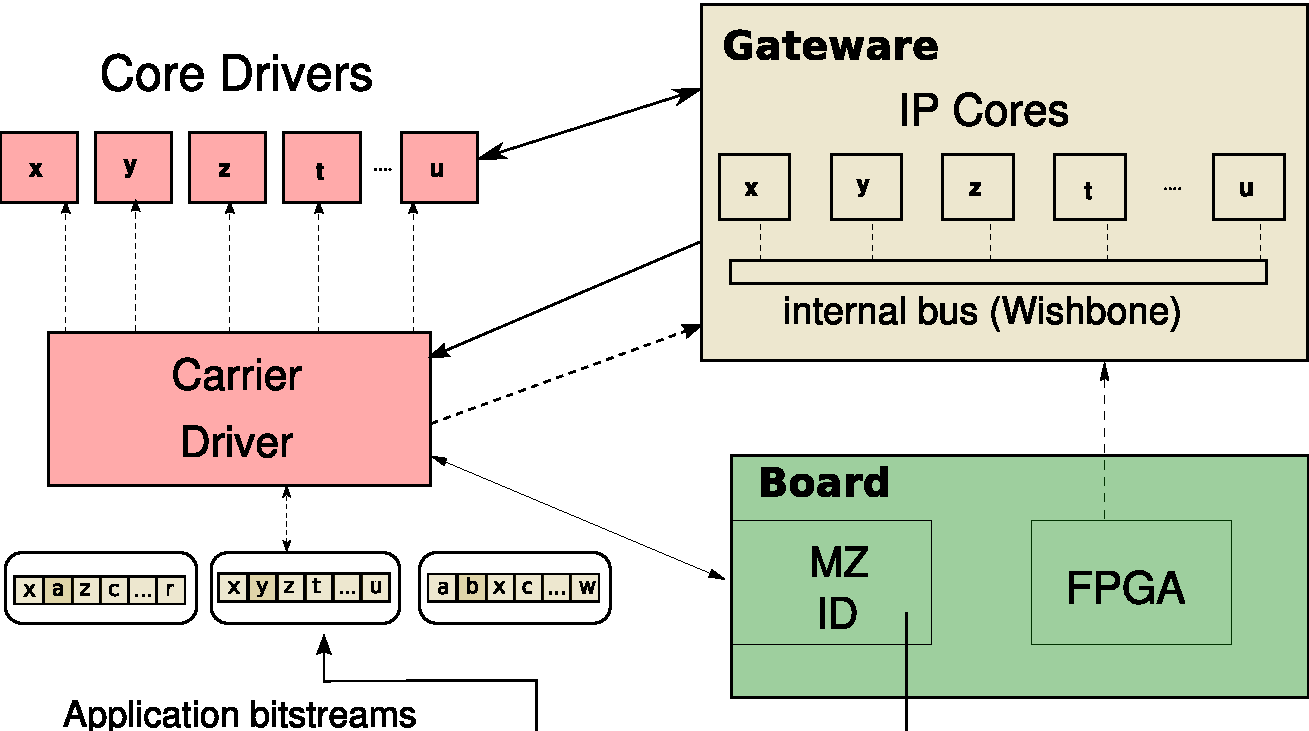
\includegraphics[height=0.8\textheight]{driverarch.pdf}
\end{frame}

% ------------------------------------------------------
\begin{frame}{How the FMC drivers start up}
\begin{itemize}
\item Identify the carrier board and initialize it.
\item Perform a basic identification of the mezzanine(s) installed in
    the FMC slot(s), and their configured applications.
\item Load the application firmware into the carrier FPGA.
\item Register a Wishbone bus with the kernel.
\item Enumerate the cores in that firmware (to wit, the
    inner blocks in figure~\ref{slow-adc}).
\item Register the devices those cores implement and install the drivers
    associated to them.
\end{itemize}
\end{frame}

\section{FMC boards}


\section{The \texttt{zio} framework}

% ------------------------------------------------------
\begin{frame}{Industrial I/O frameworks}

\pause
\begin{block}{In Linux staging area}
\begin{itemize}
\item Comedi
\item IIO
\end{itemize}
\end{block}

\pause
\begin{block}{Drawbacks}
\begin{itemize}
\item do not suit our needs
\item interfaces are cumbersome
\end{itemize}
\end{block}

\pause
\begin{block}{Then \texttt{zio} comes}
\begin{itemize}
\item Alessandro Rubini and Federico Vaga, main developers
\item Designed \emph{ab initio} for upstream integration
\item See under \url{http://www.ohwr.org/projects/zio}
\end{itemize}
\end{block}

\end{frame}

% ------------------------------------------------------

% ------------------------------------------------------
\begin{frame}
\frametitle{\texttt{zio} features}

The \texttt{zio} framework is designed to flexibly support the following
aspects:
\begin{itemize}
\item Digital and analog input and output.
\item One-shot and streaming (buffered) data acquisition or waveform play.
\item Resolution.
\item Sampling rate.
\item Buffer management and timing for streaming conversion.
\item Support for DMA.
\item Calibration, offset and gain.
\item Bit grouping in digital I/O.
\item Timestamping.
\item Triggering of acquisition/output.
\item Potential to integrate in the main tree.
\end{itemize}

\end{frame}

% ------------------------------------------------------
\begin{frame}
\frametitle{\texttt{zio} concepts}

\begin{block}{\texttt{zio} abstractions}
\begin{itemize}
\item[devices] victims of our device drivers, contain channels
\item[channels] basic I/O units
\item[channel sets] group channels to be triggered (acquire, output)
	simultaneously
\item[buffers] for input and output buffering, of course
\item[triggers] cause acquisitions to occur
\end{itemize}
\end{block}

\end{frame}

% ------------------------------------------------------
\begin{frame}
\frametitle{Typical \texttt{zio} input data flow}
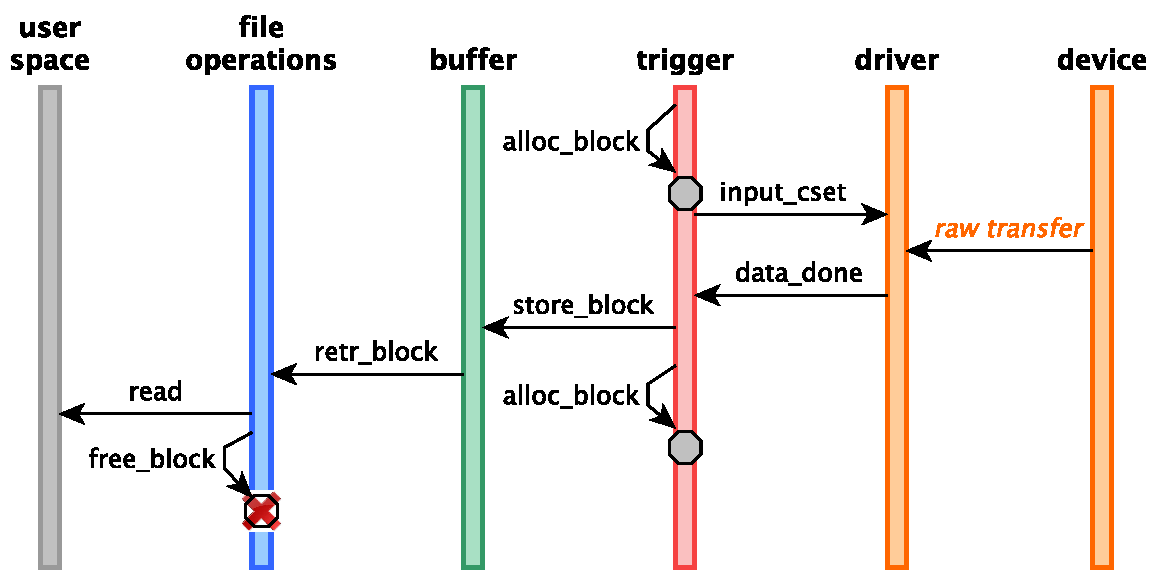
\includegraphics[height=0.8\textheight]{flow-temp-in.pdf}
\end{frame}

% ------------------------------------------------------
\begin{frame}
\frametitle{Typical \texttt{zio} output data flow}
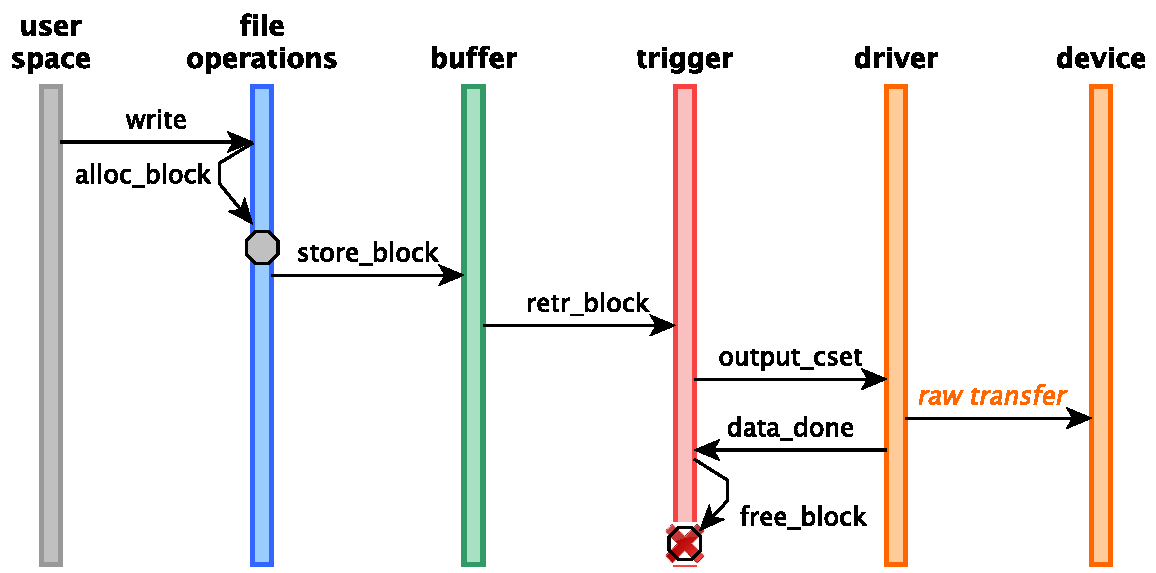
\includegraphics[height=0.8\textheight]{flow-temp-out.pdf}
\end{frame}

% ------------------------------------------------------
\begin{frame}{Next candidates for (\texttt{zio}) integration}

And for mainstream integration as well...
\pause
CERN-developed drivers for good old beasts
\begin{itemize}
\pause
\item Struck SIS33xx ADCs
\pause
\item Tews TPCI200/TVME200 carries plus IPOCTAL serial boards
\pause
\item all the CERN BE/CO-supported FMC boards in the Open Hardware Repository
\pause
\item timing receivers, White Rabbit, etc.
\end{itemize}
\end{frame}

\section{Conclusions and The Ultimate Goal}

% ------------------------------------------------------
\begin{frame}{Let's summarize}

\begin{itemize}
\pause
\item Accelerator control systems require managing a complex and
    diverse zoo of hardware devices
\pause
\item Open Hardware makes for a much more manageable design and 
    production way
\pause
\item It is proven to work in practice
\pause
\item Both for a big project like White Rabbit and for the myriad
    of heterogeneous devices linked to it
\pause
\item The software side cannot simply live without the Open Software
    model
\pause
\item Especially the Linux kernel! Thanks for the device model and
    the I/O frameworks
\end{itemize}
\end{frame}

\end{document}
